\documentclass[a4paper]{article}

%% Language and font encodings
\usepackage{polski}
\usepackage[polish]{babel}
\usepackage[utf8x]{inputenc}
\usepackage[T1]{fontenc}
\usepackage{pdfpages}
\usepackage{indentfirst}

% Adjust penalties
\brokenpenalty=1000
\clubpenalty=1000
\widowpenalty=1000

%% Sets page size and margins
\usepackage[a4paper,top=3cm,bottom=2cm,left=3cm,right=3cm,marginparwidth=1.75cm]{geometry}

%% Useful packages
\usepackage{amsmath}
\usepackage{graphicx}
\usepackage[colorinlistoftodos]{todonotes}
\usepackage[colorlinks=true, allcolors=blue]{hyperref}

\renewcommand\thesection{\arabic{section}.}
\renewcommand\thesubsection{\arabic{section}.\arabic{subsection}.}
\renewcommand\thesubsubsection{\arabic{section}.\arabic{subsection}.\arabic{subsubsection}.}

\newcommand{\code}{\texttt}

\title{The Project Game}
\author{
Adam Bernat \\
Tomasz Chudzik \\
Marcin Godniak \\
Adrian Sadłocha \\
Michalina Tumialis
}



\begin{document}
\maketitle
\tableofcontents
\newpage

\listoftodos
\newpage

\section{Cel projektu}

Celem jest zaplanowanie oraz~implementacja gry symulującej pracę w środowisku projektowym.
Szczególny nacisk kładziony jest na badanie wpływu zachowań poszczególnych graczy (tj. członków rywalizujących zespołów) na efektywność.

\section{Opis gry}

Gra jest toczona przez dwa rywalizujące zespoły.
Oba zespoły składają się z~wielu graczy oraz~z~jednego wyróżnionego -- lidera zespołu.

Gra jest rozgrywana na prostokątnej planszy, która jest podzielona na trzy strefy: dwie strefy celu (po jednej na każdą drużynę) oraz~na~środkową strefę -- strefę zadań.
Zadania do przedsięwzięćia przez zespoły są reprezentowane przez kawałki.
Są one umieszczane w strefie zadań, z~której to muszą zostać podniesione przez graczy, a następnie zaniesione do strefy celu.
W strefie celu gracz jest w stanie stwierdzić, czy podniesiony kawałek był fałszywką, czy nie.

Każdy gracz przechowuje własny stan gry.
Gracze mogą się ze sobą komunikować, wykazując różne wzorce zachowań.
Prawdziwy stan gry jest przechowywany przez mistrza gra, który jest odpowiedzialny za wygenerowanie planszy oraz~umieszczanie nowych kawałków w strefie zadań.
Wszelka komunikacja pomiędzy mistrzem gry a graczami odbywa się poprzez serwer komunikacyjny.

\section{Zasady gry}

\section{Słowniczek pojęć}

\todo{Słowniczek pojęć}

\section{Aktorzy}

\todo{Aktorzy}

\subsection{Reguły}

\todo{Reguły}

\subsection{Możliwe akcje}

\todo{Możliwe akcje}

\subsubsection{Przypadki użycia}

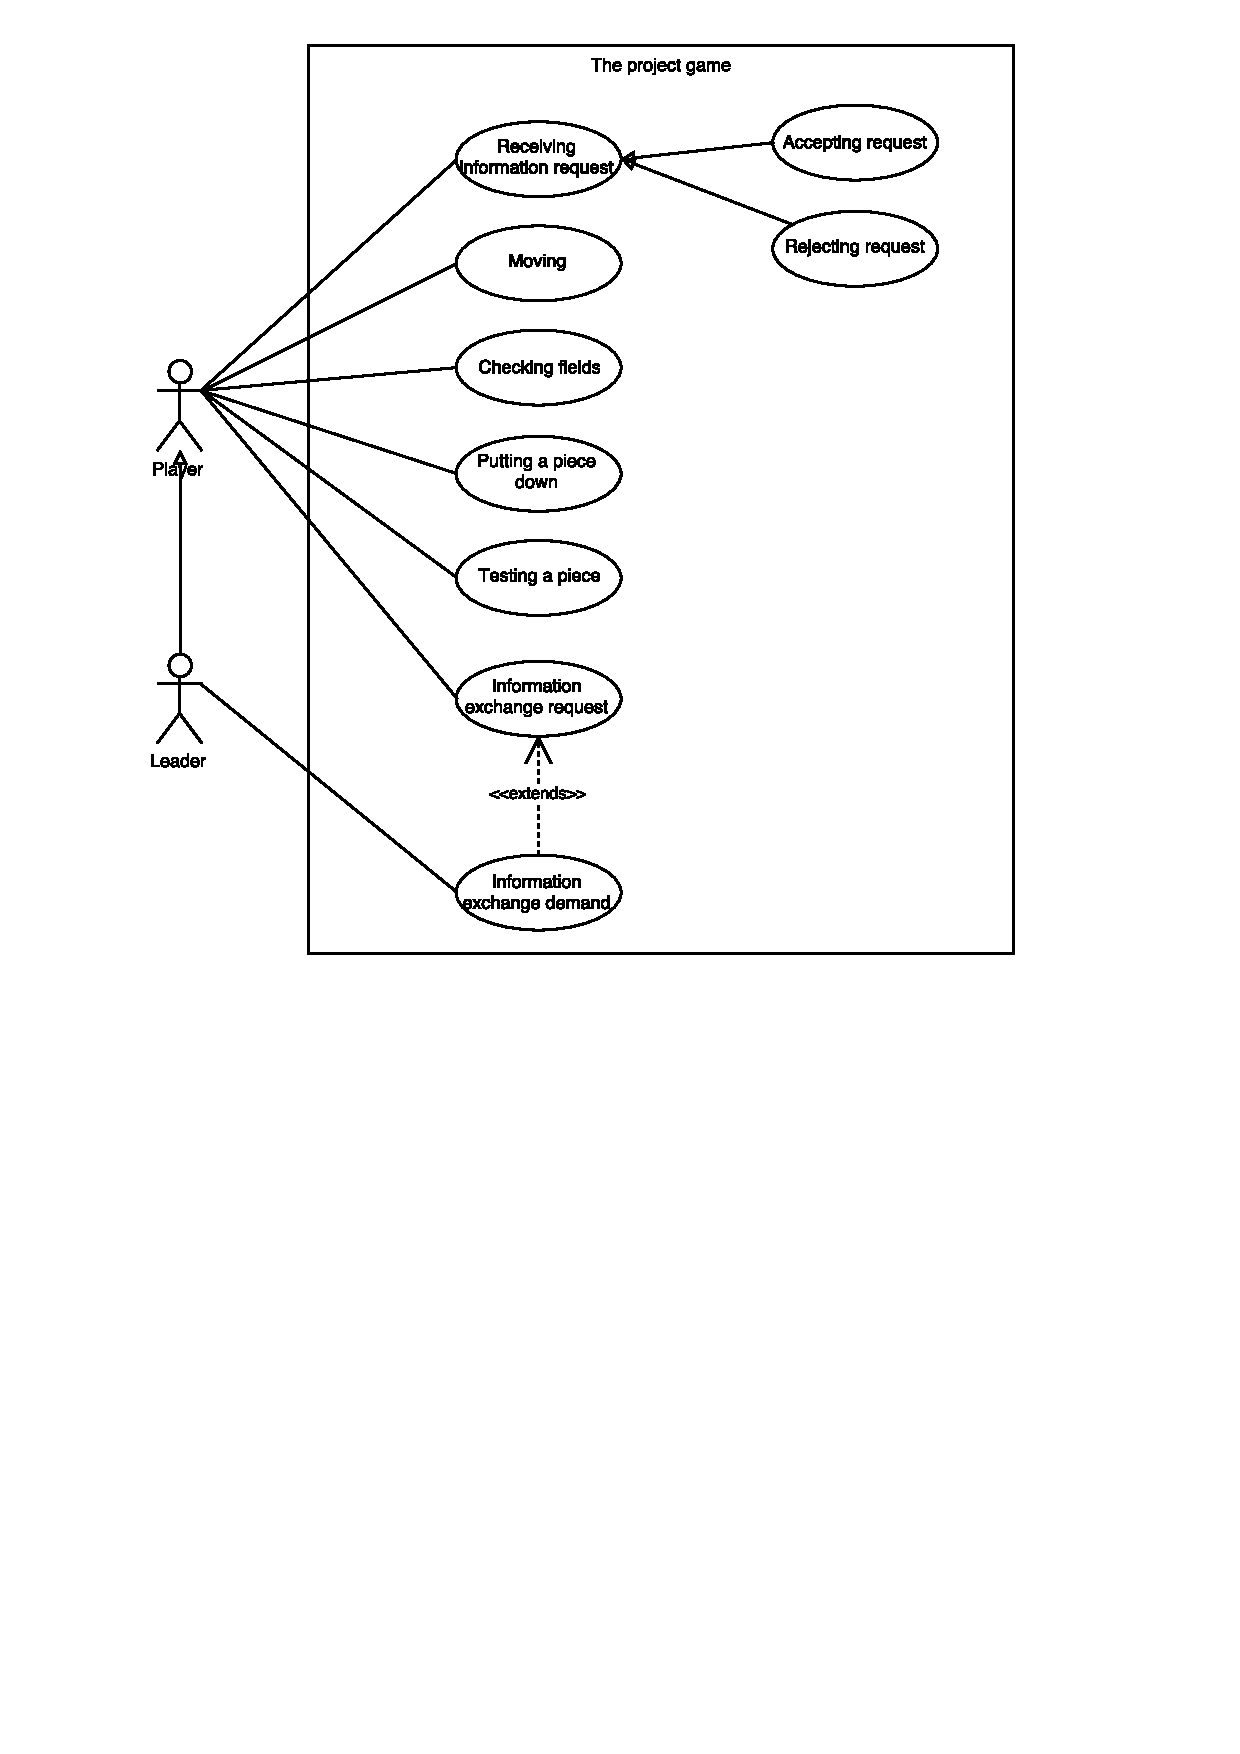
\includepdf[pages={1}]{przypadki_uzycia_gracz_lider.pdf}
Gracz może otrzymać prośbę o wymianę informacji.
Prośba może zostać zaakceptowana lub~odrzucona.
Wyjątkiem jest prośba o wymianę informacji od lidera zespołu -- ta nie może zostać odrzucona.

Gracz może poruszać się w jednym z~czterech kierunków (góra, dół, prawo, lewo).
Nie może jednak wejść na pole celu przeciwnego zespołu.

Gracz ma również do dyspozycji następujące akcje: sprawdzenie pól dookoła, podniesienie kawałka z~aktualnego pola, przetestowanie kawałka (o ile gracz znajduje się w strefie celu).
Ponadto, gracz może wysłać prośbę o wymianę informacji do innego gracza.
W szczególności, może zarządać wymiany informacji od lidera.

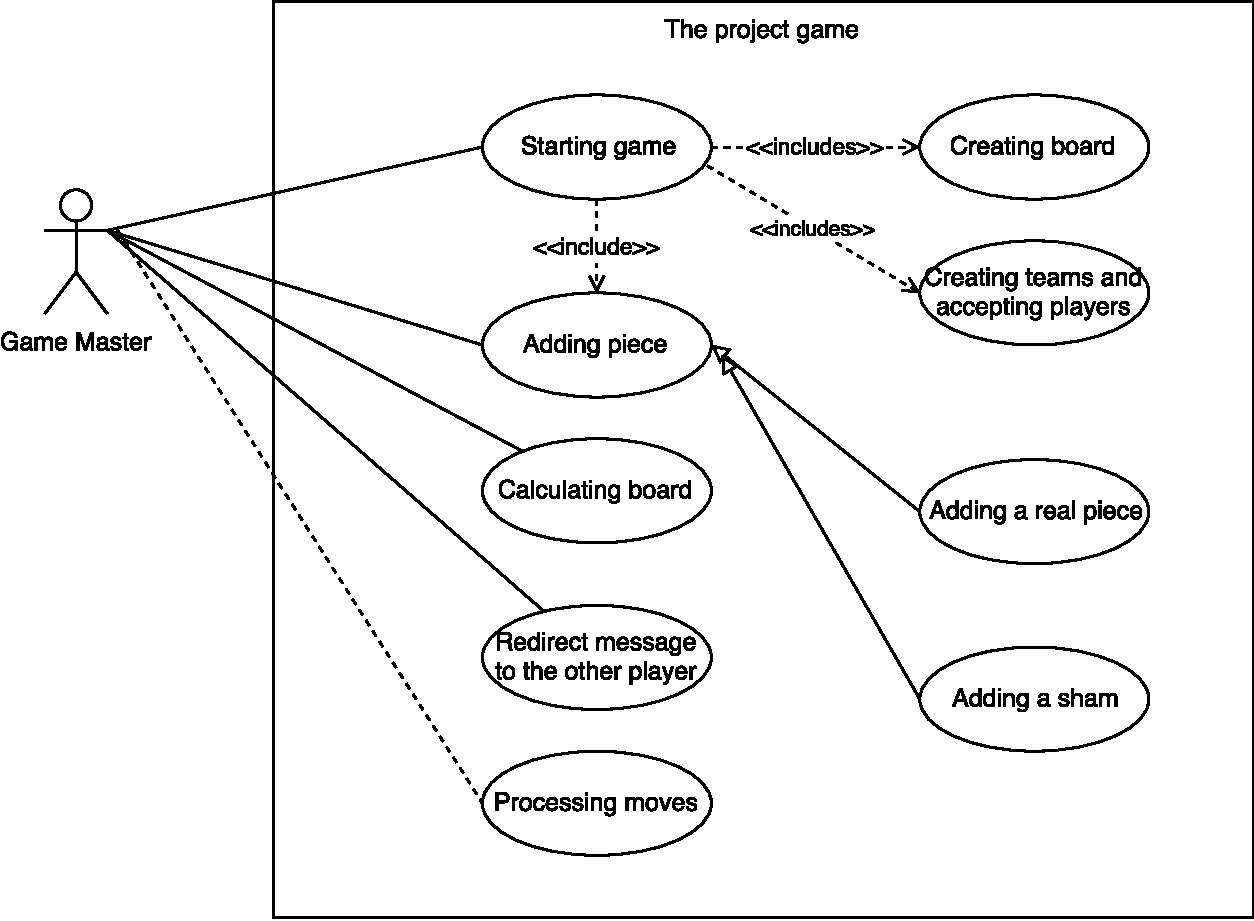
\includepdf[pages={1}]{przypadki_uzycia_gm.pdf}

Mistrz gry rozpoczyna grę, tj. generuje planszę oraz~czeka (i akceptuje) łączących się graczy.
Następnie -- podczas gry -- dodaje kawałki (fałszywe lub nie) do strefy zadań; przelicza odległości do najbliższych kawałków; przekierowuje wiadomości pomiędzy graczami; oraz~przetwarza ruchy graczy.

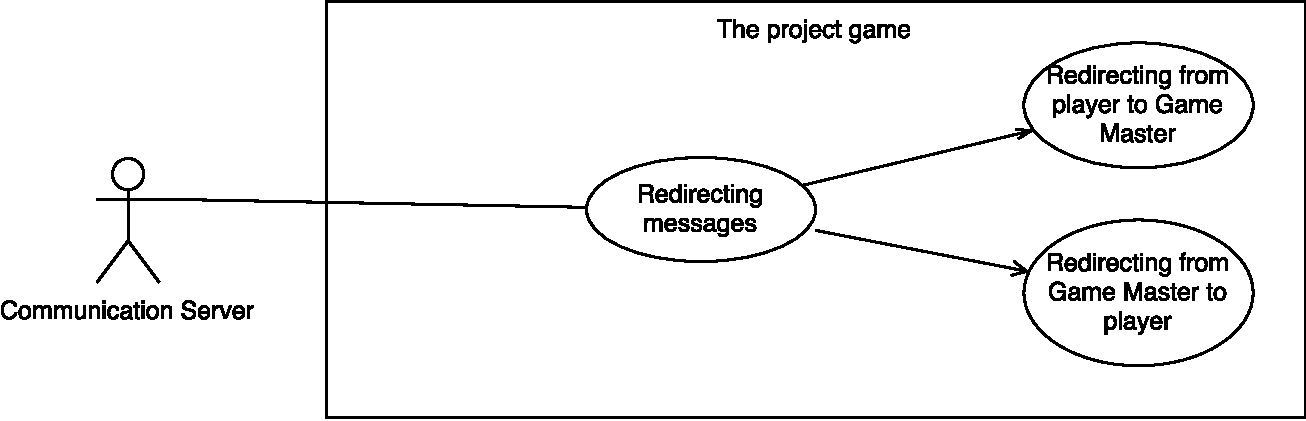
\includepdf[pages={1}]{przypadki_uzycia_cs.pdf}

Serwer komunikacyjny odpowiada za przekierowywanie wiadomości pomiędzy graczami a mistrzem gry.

\section{Możliwości konfguracyjne}

\todo{Możliwości konfguracyjne}

\section{Uruchamianie aplikacji}

\todo{Uruchamianie aplikacji -- jak będzie uruchamiana, co będzie wynikiem, skąd jest czytana konfiguracja etc.}

\section{Wymagania niefunkcjonalne}

\todo{FURPS -- ile graczy obsługiwanych maksymalnie, co w przypadku problemów na łączach (rozłączenie gracza itp.)}

\section{Opis architektury}

\subsection{Diagram klas}
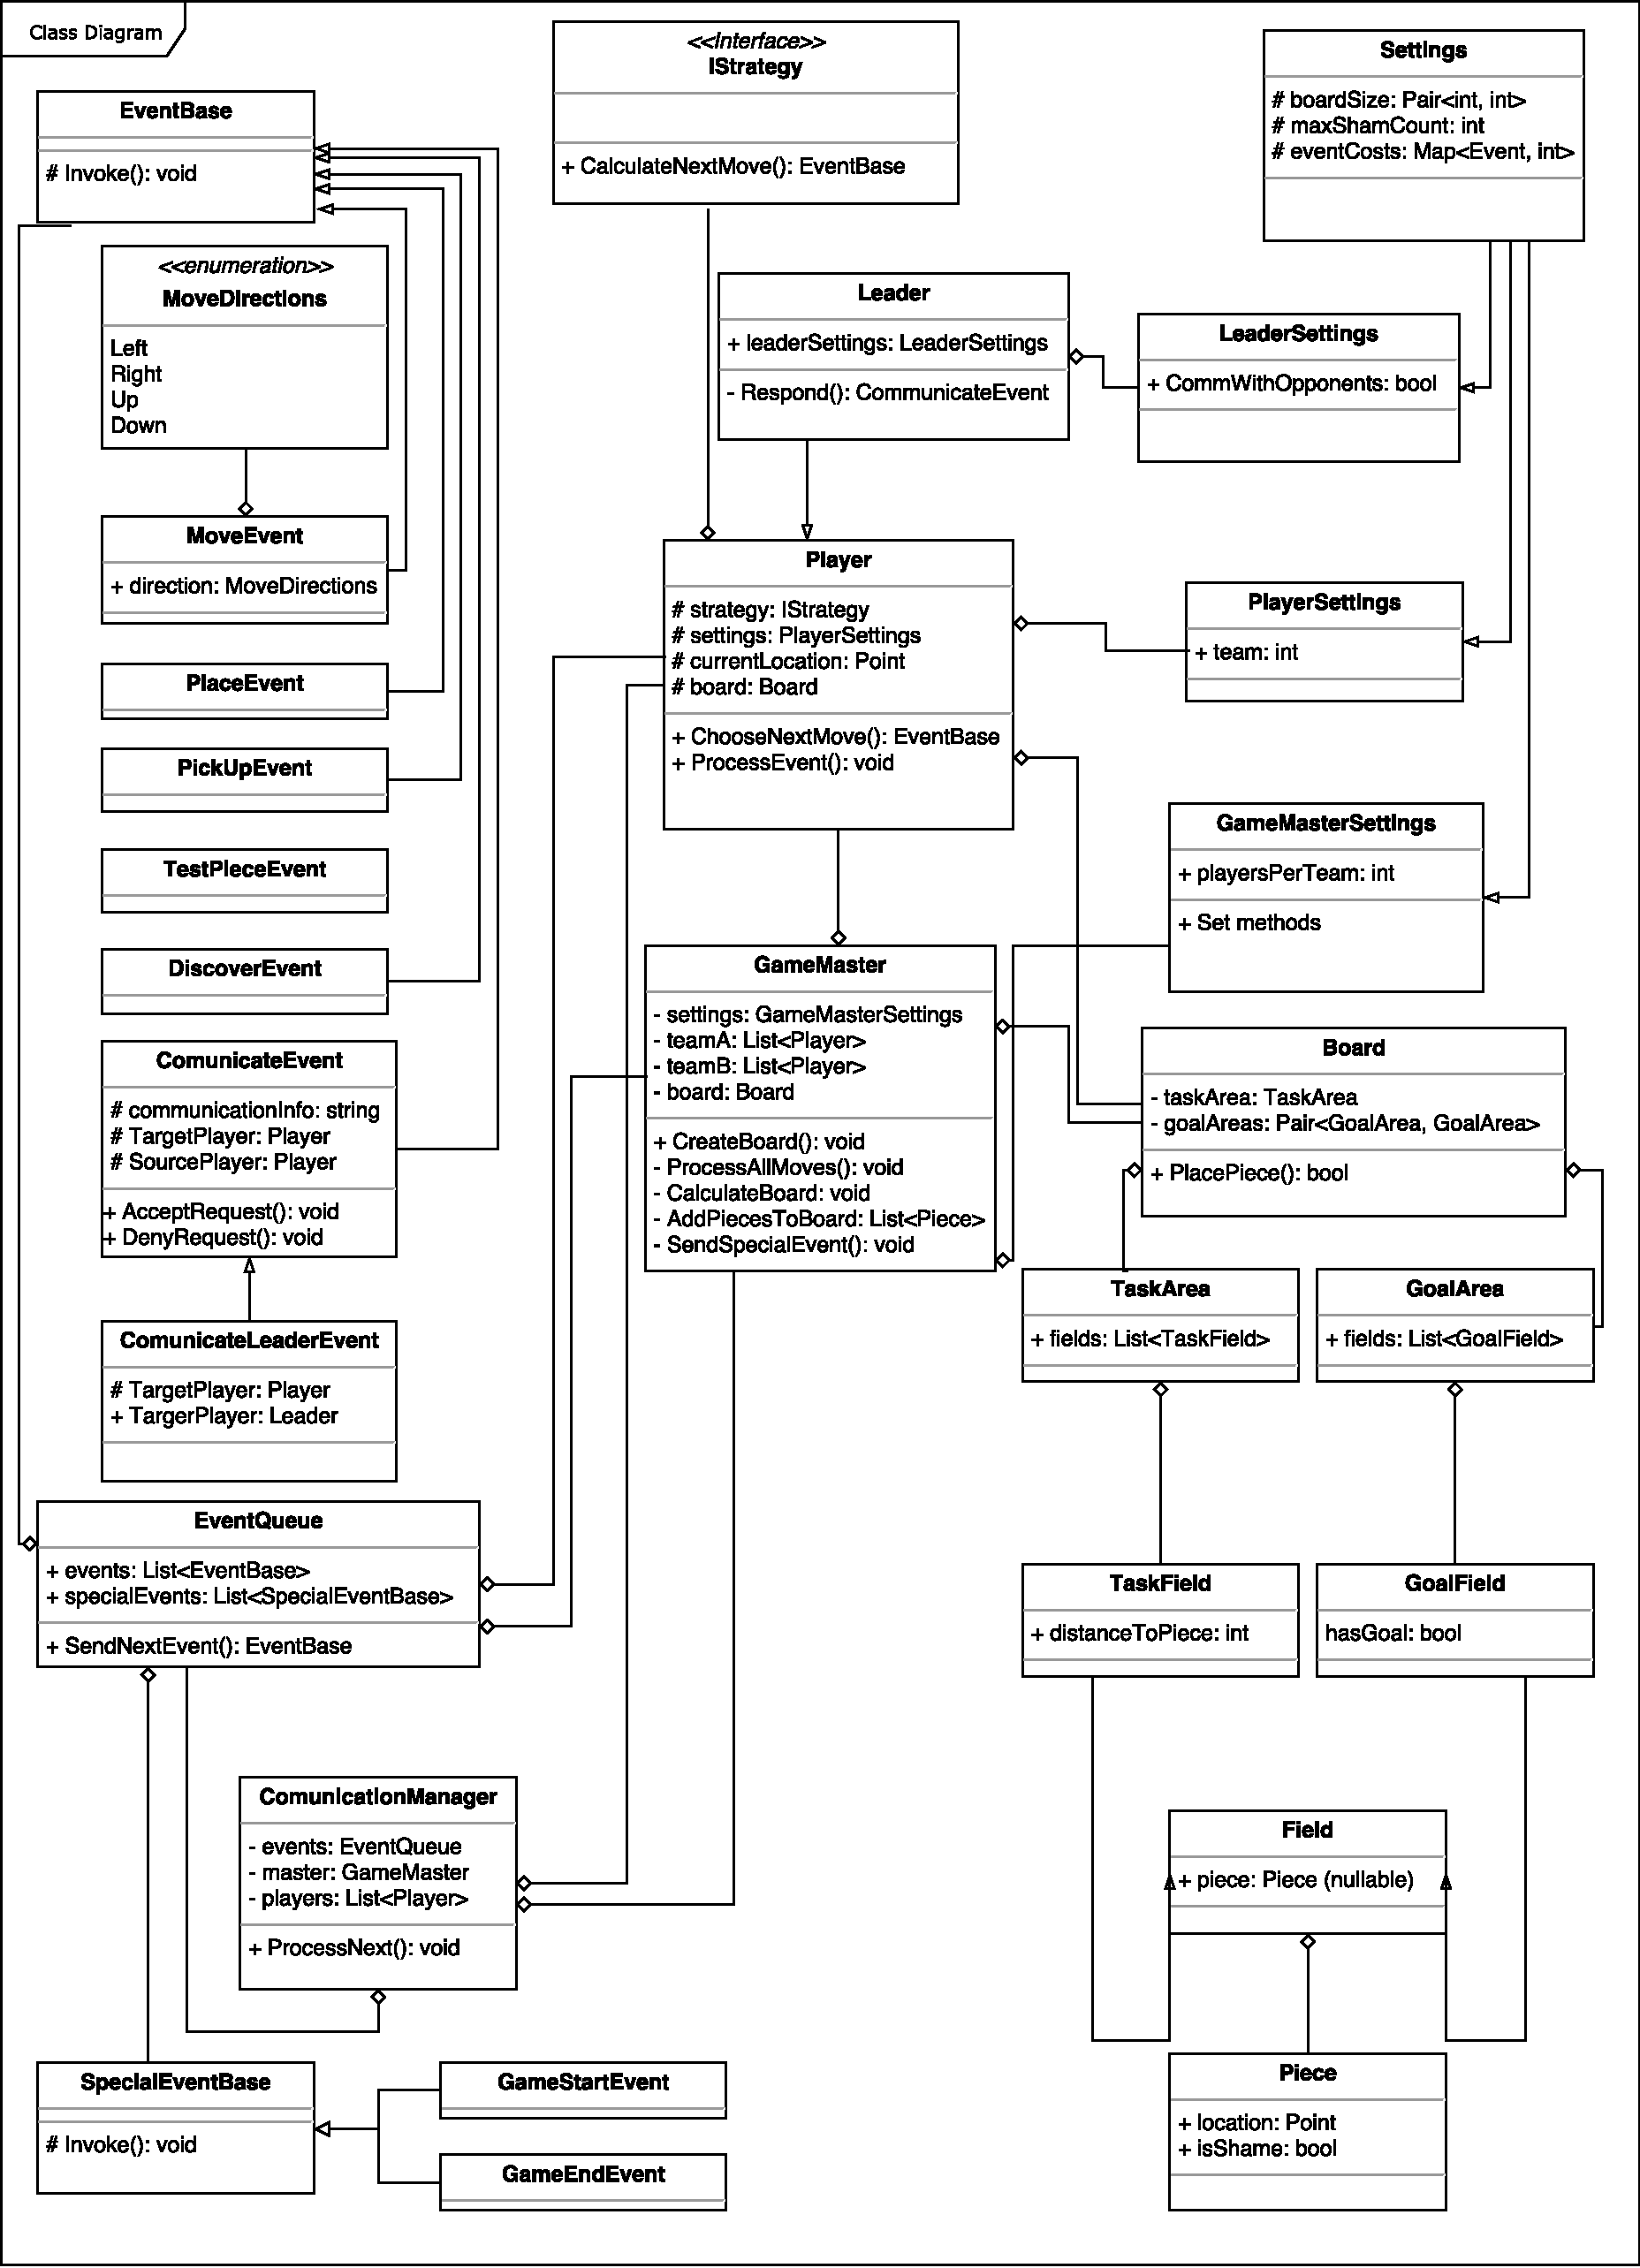
\includepdf[pages={1}]{diagram_klas.pdf}

Klasa gracza zawiera pole strategii, odpowiedzialnej za wyliczanie kolejnych ruchów.
Ponadto, klasa przechowuje pole ustawień (numer zespołu, rozmiar planszy, maksymalna liczba dopuszczalnych fałszywek oraz~mapę kosztów poszczególnych ruchów).
Gracz przechowuje również swoja aktualną pozycję na planszy oraz~referencję do obiektu planszy.
Gracz może wybrać swój następny ruch oraz~może przetwarzać nadchodzące wydarzenia.
Lider jest specjalnym rodzajem gracza, mającym dodatkowe ustawienie -- czy musi się komunikować z~przeciwną drużyną, czy nie.

\hfill 

W grze występują następujące wydarzenia:
\begin{itemize}
	\item \code{MoveEvent} -- zawiera kierunek ruchu (lewo, prawo, góra, dół);
	\item \code{PickUpEvent} oraz~\code{PlaceEvent} -- wydarzenia mające miejsce, gdy gracz kolejno podnosi lub~odkłada kawałek;
	\item \code{TestPieceEvent} -- akcja sprawdzania przez gracza, czy kawałek jest fałszywką, czy nie;
	\item \code{DiscoverEvent} -- sprawdzenie przez gracza pól dookoła;
	\item \code{CommunicateEvent} -- prośba o wymianę informacji pomiędzy dwoma graczami (prośba o wymianę informacji może zostać zaakceptowana lub odrzucona; jedynie lider ma obowiązek odpowiadania na prośby);
\end{itemize}

Wydarzenia są umieszczanie w kolejce \code{(EventQueue}), która zawiera przedstawione wyżej wydarzenia oraz~dwa specjalne: \code{GameStartEvent} tudzież~\code{GameEndEvent}.

\hfill

Mistrz gry jest klasą odpowiedzalną za stworzenie planszy, przeliczanie stanu gry, dodawania kawałków do planszy, przetwarzenie wszytkich ruchów graczy oraz~za wysyłanie specjalnych wydarzeń, takich jak informacja o początku lub końcu gry.
Ta klasa zawiera referencje do obu zespołów, planszy; przetrzumuje rownież obiekt ustawień z~informacjami takimi jak liczba graczy w drużynie.

Komunikacja pomiędzy graczami a mistrzem gry odbywa się za~pośrednictwem serwera komunikacyjnego.
Przetrzumuje on listę wydarzeń, graczy oraz~referencję na mistrza gry.

Podstawowa klasa ustawień (Settings) zawiera informacje o rozmiarach planszy (za pomocą pary liczb całkowitoliczbowych zdefiniowana jest szerokość i~wysokość), maksymalnej liczbie fałszywek.
Ponadto, przechowuje mapę kosztów poszczególnych akcji.

Klasa planszy zawiera trzy strefy: jedną strefę zadań oraz~dwie strefy celu.
Strefa zadań przechowuje pola, na których mogą znajdować się kawałki.
Pola te zawierają odległość do najbliższego kawałka.
Każda strefu celu zaś przechowuje pola, które mogą być częścią celu.
Odkrywa się je, poprzez odkładanie na nich prawdziwych kawałków.
Pola celu zawierają zmienną typu logicznego, która określa, czy jest to część zadania.

Klasa kawałków przechowuje swoją lokalizację na planszy oraz~pole logiczne informujące o~prawdziwości kawałka.

\newpage
\section{Diagram aktywności}
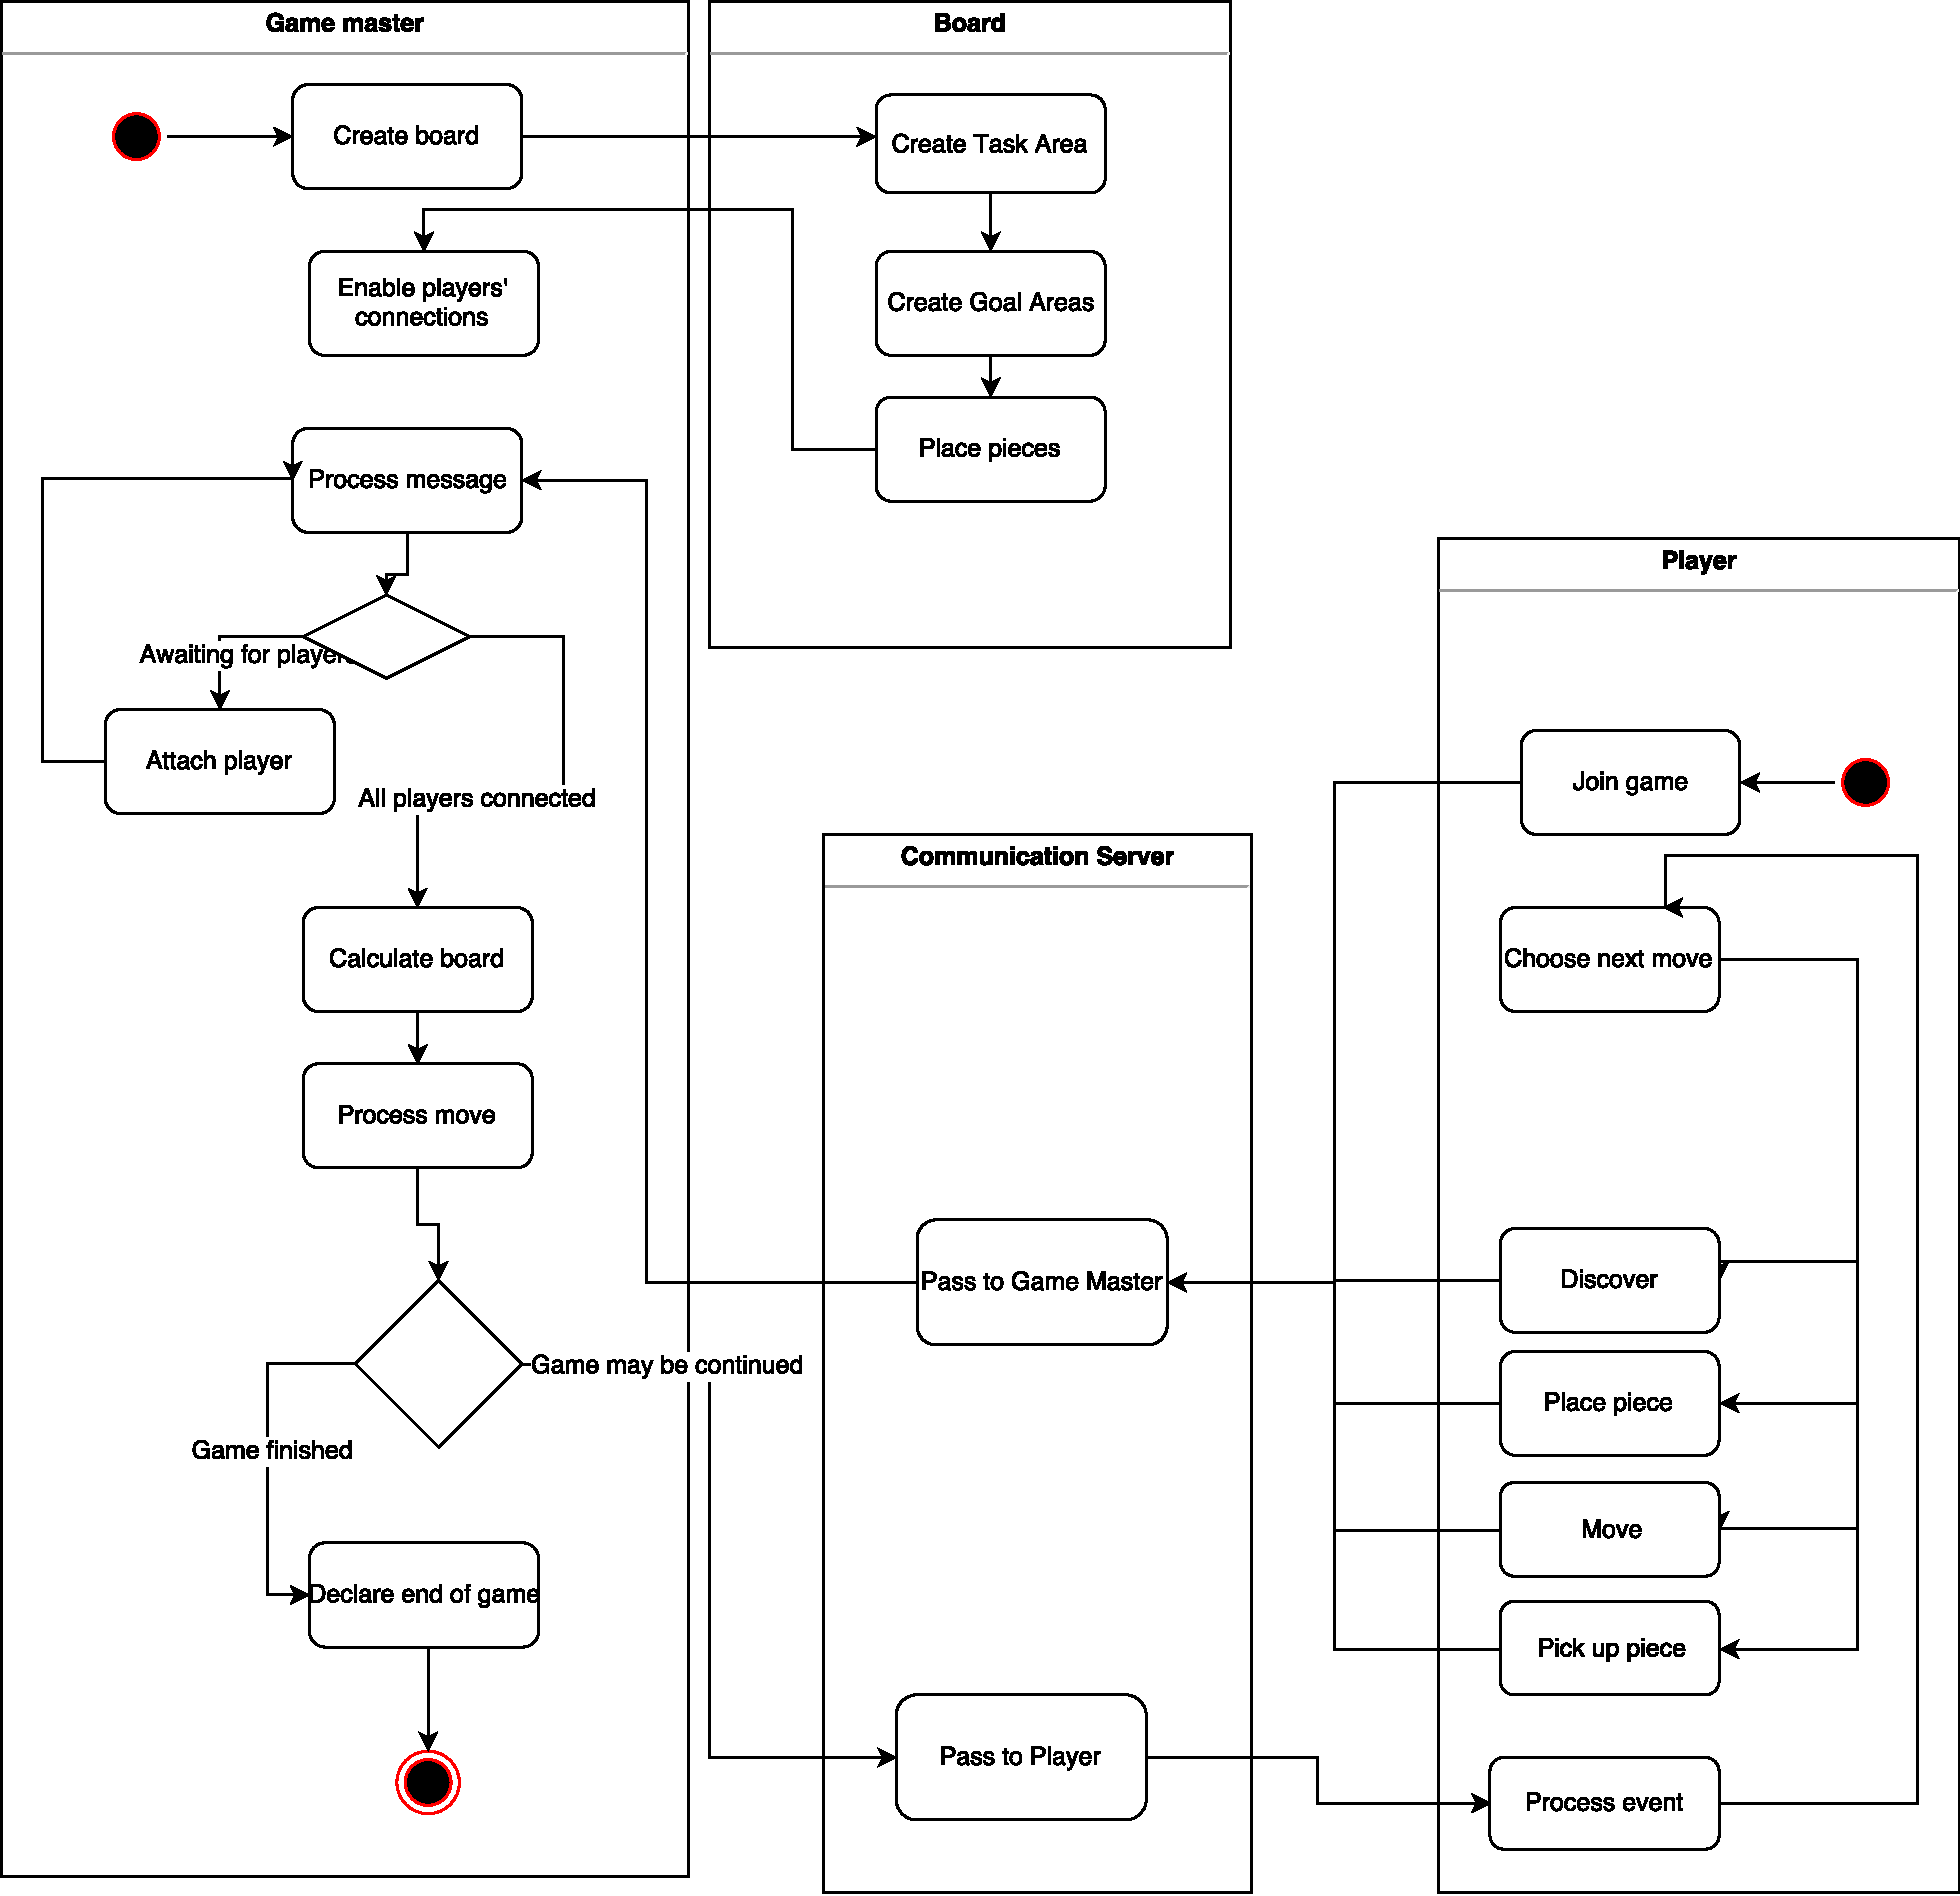
\includepdf[pages={1}]{diagram_aktywnosci.pdf}
Po rozpoczęciu gry, mistrz gry tworzy planszę: strefę zadań; strefy celów; umieszcza kawałki.
Następnie czeka aż gracze się połączą.

Po podłączeniu wszystkich graczy, mistrz gry utrzymuje stan planszy oraz~obsługuje ruchy graczy.
Kiedy gra zostanie zakończona, informuje graczy o końciu rozgrywki.

Gracze mogą dołączyć do gry i~wykonywać ruchy: odkrywanie pól dookoła; ruch w jednym z~czterech kierunków; podniesienie lub odłożenie kawałka.
Ruchy są przekazywane do mistrza gry (i odpowiedzi są przekazywane z~powrotem do gracza) za~pośrednictwem serwera komunikacyjnego.

\newpage
\section{Diagram stanów}
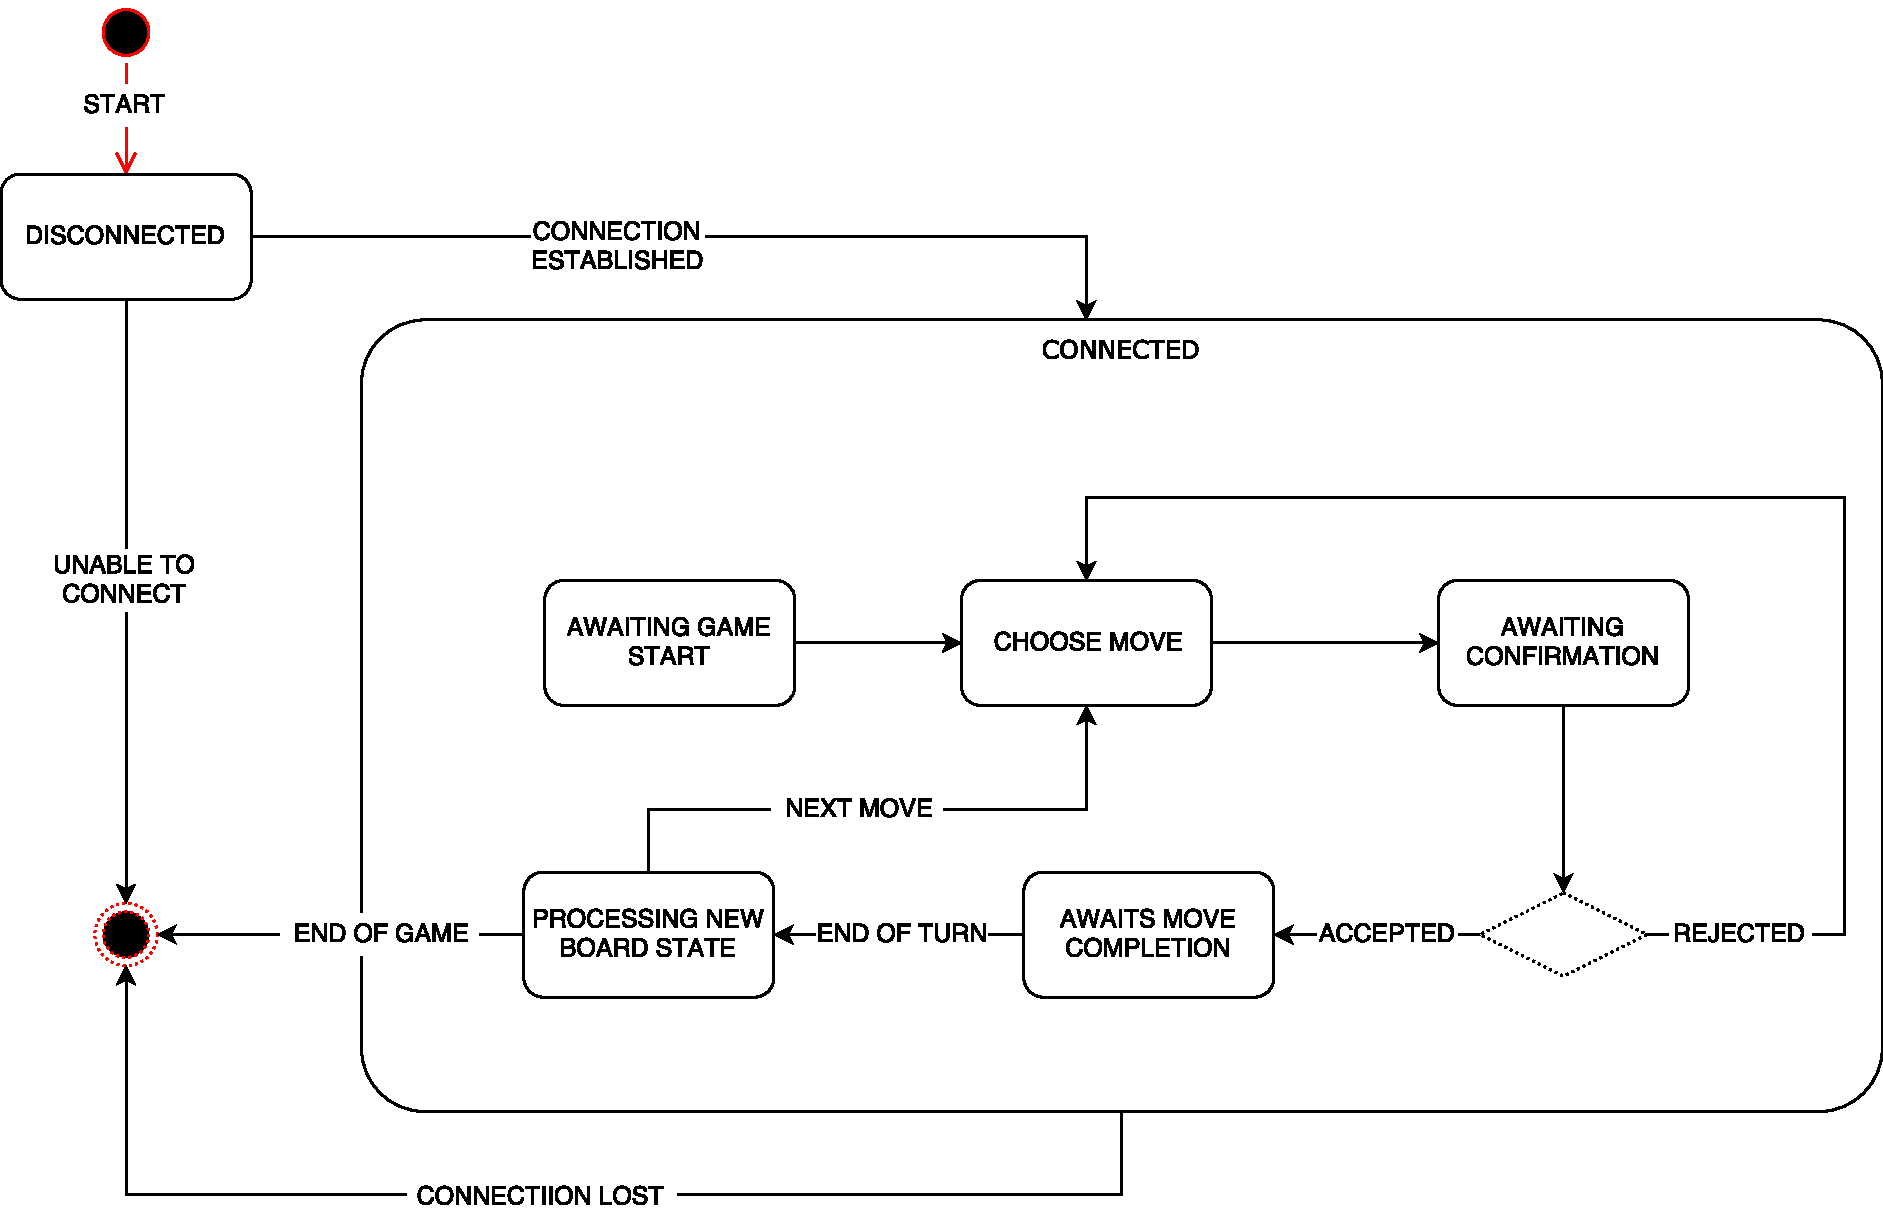
\includepdf[pages={1}]{state_diagram_player.pdf}

Na początku, gracz jest w stanie rozłączonym i~próbuje połączyć się z~grą.
Jeśli się to nie uda, kończy działanie.

Jeśli jednak połączenie zostanie nawiązane, to gracz oczekuje na rozpoczęcie gry.
Po rozpoczęciu gry, gracz -- w pętli -- wykonuje ruch, oczekuje odpowiedzi, czeka na zakończenie ruchu, przetwarza nowy stan gry.
Jeśli ruch zostanie odrzucony przez mistrza gry, gracz od razu próbuje wykonać kolejny ruch.

Jeśli w którymś momencie gracz otrzyma wiadomość o zakończeniu gry (lub utraci połączenie), kończy działanie.

\section{Protokół komunikacyjny}

\todo{Opis słowny komunikacji}

\subsection{Diagram sekwencji}
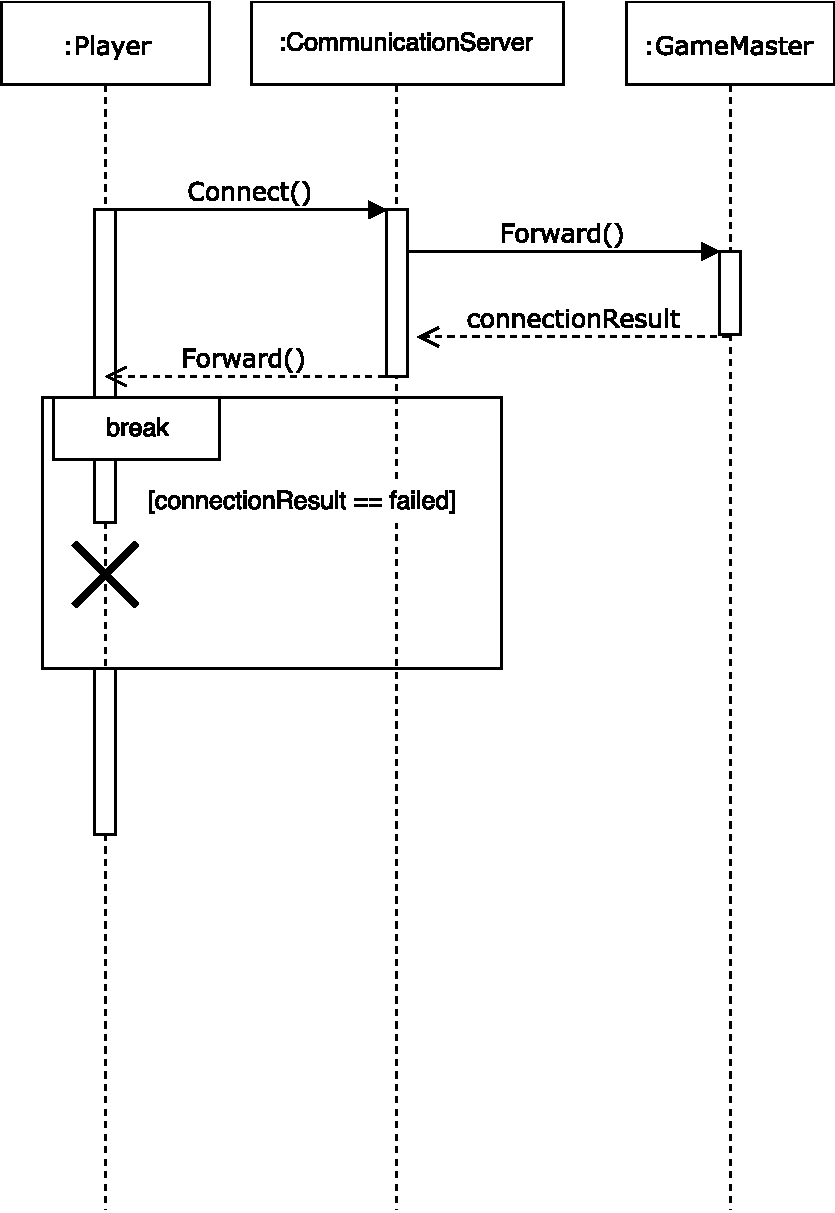
\includepdf[pages={1}]{sekwencje1.pdf}

Najpierw gracz wywołuje metodę \code{Connect()} i~czeka na odpowiedź od serwera komunikacyjnego, który to przekierowuje zapytanie do mistrza gry i~czeka na odpowiedź, którą przekazuje do gracza.
Jeśli gracz zostanie dodany do gry, bierze udział w grze.
W przeciwnym przypadku kończy działanie.

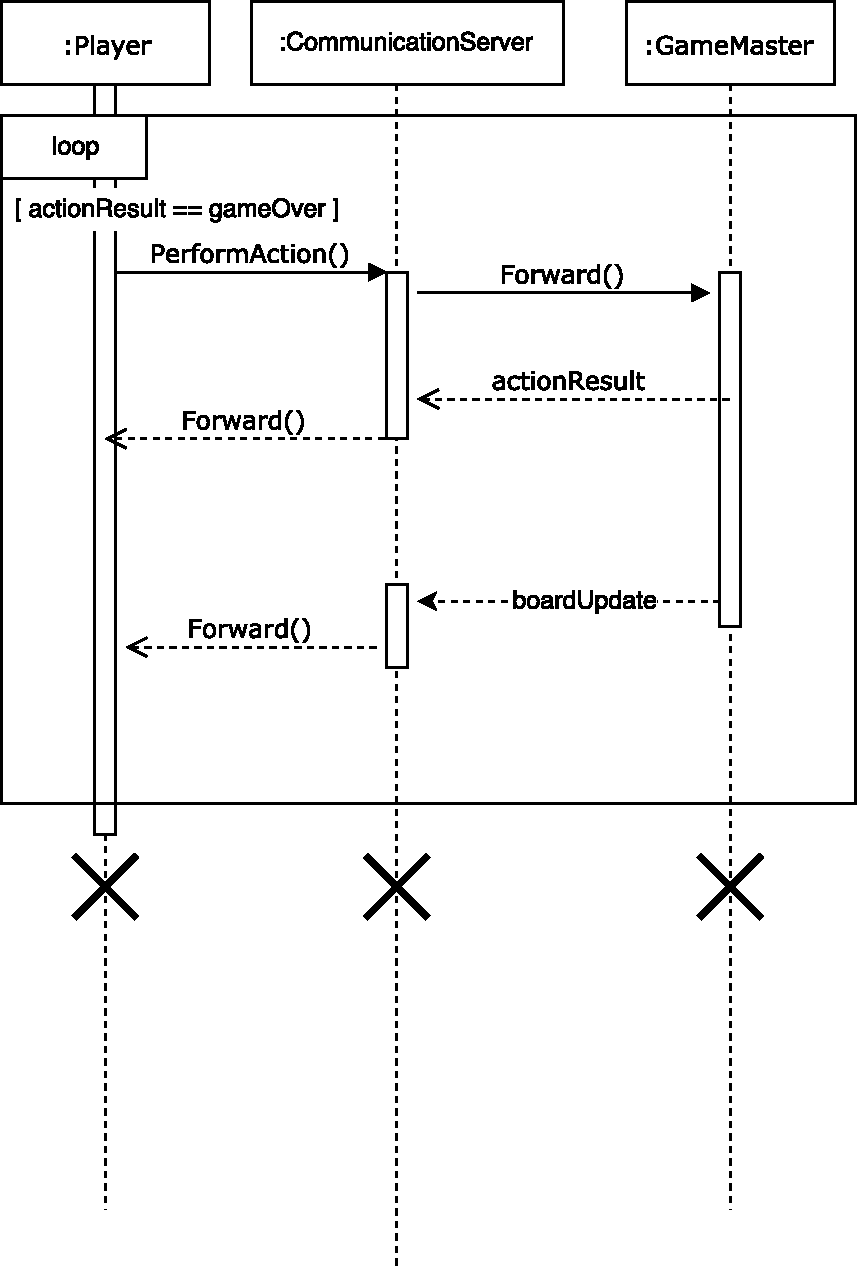
\includepdf[pages={1}]{sekwencje2.pdf}

Gracz wykonuje ruchy w pętli, która kończy się, gdy dostanie odpowiedź (z serwera komunikacyjnego) z~komunikatem ,,koniec gry''.
Serwer komunikacyjny dostaje informacje o ruchach wykonywanych przez graczy i~przekazuje je do mistrza gry.
Następnie czeka na odpowiedź, którą przekazuje do gracza.
Ponadto, otrzymuje informacje o komunikatach od mistrza gry, które przekazuje graczom.

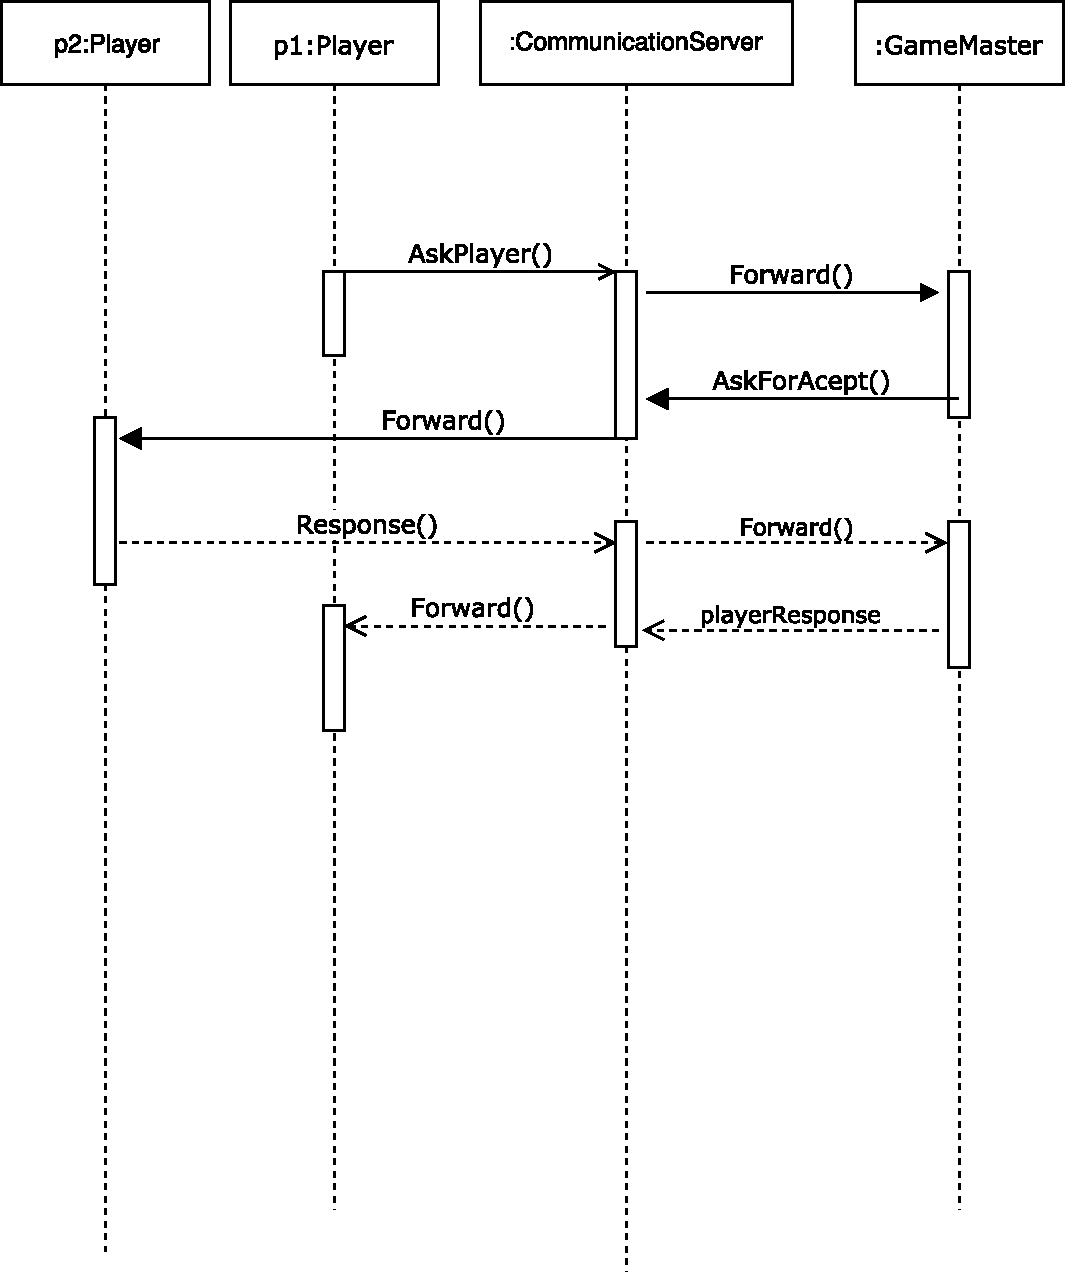
\includepdf[pages={1}]{sekwencje3.pdf}

Komunikacja pomiędzy graczami odbywa się za~pośrednictwem serwera komunikacyjnego i~mistrza gry.

Kiedy gracz \code{p1} chce skomunikować się z~graczem \code{p2}, najpierw wysyła wiadomość do serwera komunikacyjnego.
Serwer komunikacyjny przekazuje zapytanie do mistrza gry, który następnie decyduje, czy taki ruch jest możliwy w danym momencie.
Jeśli tak, to mistrz gry wysyła zapytanie (zawierające pole nadawcy, czyli gracza \code{p1}) do \code{p2}.
Po otrzymaniu tej wiadomości (ponownie: za~pośrednictwem serwera komunikacyjnego), gracz \code{p2} decyduje o odpowiedzi (akceptacji lub odrzuceniu) i~wysyła ją. Odpowiedź wędruje przez serwer komunikacyjny do mistrza gry, ponownie do serwera komunikacyjnego, aż trafi do gracza \code{p1}.

\subsection{Struktura wiadomości}

\todo{Struktura wiadomości -- XML/JSON?}

\section{Opis sytuacji wyjątkowych}

\subsection{Utrata łączności z graczem}
\subsection{Utrata łączności z serwerem komunikacyjnym}
\subsection{Utrata łączności z mistrzem gry}

\end{document}
